\chapter{Neural Networks}
\label{cha:neural_networks}
\epigraph{In the recent years Neural Networks (NN) have solved more and more
  tasks that have previously been too difficult or simply too tedious to solve
  with traditionally coded algorithms. They have been successfully applied to a
  variety of problems such as pattern recognition, image classification and
  prediction.  As the NN algorithms learn from data, they seem to be good
  candidates for finding anomalies without any a prior knowledge about the
  given dataset, as long as it is big enough. By applying online learning
  algorithms that learn and adapt continuously it should in theory be possible
  to create an automated, adaptive outlier detection.\\ This chapter describes
  the mechanics of NNs from the ground up. Starting with the widely used
  \emph{feedforward networks} (FNN), we go on to \emph{recurrent neural nets}
  (RNN). Similar to biological neural networks, they have cyclic connections,
  and are capable of processing sequences. After that, a special kind of RNN is
  introduced, that dramatically cuts computational costs and solves some
  notorious problems that arise during RNN training. In addition to the general
  difficulty of training NNs, they often rely on hyper-parameters, that are
  typically set by manually tuning the network.  This chapter is closed with a
  brief description of hyper-parameter optimization techniques which were used
  to automate this task.
}

\section{Feedforward Neural Networks}
\label{sec:feedforward_neural_networks}

The idea for artificial neural networks (ANN) is based on the human brain,
which is a highly complex, non-linear, and parallel computer.  Just like the
brain, ANNs are constructed from small units that are connected to each other
with weights. In analogy to its biological counterpart these units are also
called \emph{neurons}. Older literature also often refers to them as
\emph{perceptrons}.  They are capable of processing and passing on incoming
information.
Traditional feedforward networks implement static input-output mappings, which
mathematically makes them pure functions of the input signals.
Figure \ref{fig:perceptron} shows a simple schematic of a single
neuron.  It generally has $n$ inputs $u_j$ and one output.  Each of the inputs
has an assigned weight $w_j$, which determines the contribution of a given
input to the output.  The output of a neuron will further be referred to as
\emph{activation} $y$:
\begin{equation}
  \label{eq:ffn_eq}
  y = \varphi \left( \sum_j (w_j u_j) + b  \right)
       = \varphi (\vec{w} \cdot \vt{u} + b).
\end{equation}
The sum over all the inputs multiplied by their weights can conveniently be
represented by a dot product.  Often a bias term $b$ is included, which can be
taken as a measure of how easy it is to activate the neuron.  The function
$\varphi$ is called activation function and can have various different forms,
from a simple binary function to an arbitrary (non-linear), monotonically
increasing function.  A frequently used activation function in FNNs is the
sigmoid function
\begin{equation}
  \sigma (z) = \frac{1}{1 + e^{-z}},
\end{equation}
which is shown in Fig.~\ref{fig:sigmoid}. To create a \emph{layer} of neurons
they are simply stacked on top of each other:
\begin{equation}
  \vt{y} = \varphi (\wmatr{} \vt{u} + \vec{b}).
\end{equation}

\begin{figure}
  \begin{minipage}{.42\textwidth}
    \centering
    \Perceptron
    \caption{Schematic of a neuron [\cite{Nielsen2015}].
    The activation function is represented by the circle.}
    \label{fig:perceptron}
  \end{minipage}
  \hspace{.02\textwidth}
  \begin{minipage}{.54\textwidth}
    \centering
    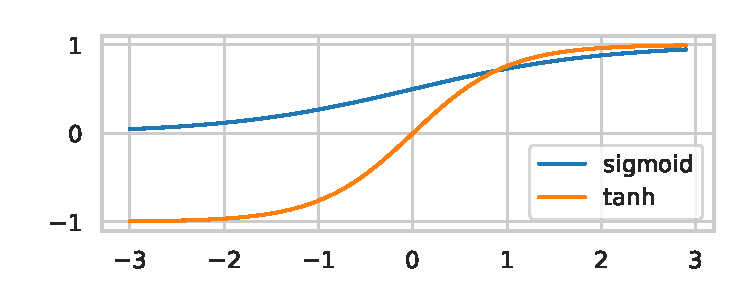
\includegraphics[width=\linewidth]{sigmoid_tanh.pdf}
    \caption{Sigmoid function $\varphi$. Typically used as an activation function
    in feedforward neural nets.}
    \label{fig:sigmoid}
  \end{minipage}
\end{figure}

The final FNN with multiple layers (such as in
Fig.~\ref{fig:feedforward_network}) is created by feeding the output of one
layer to another one until the last layer of the network is reached.  The
\emph{universal approximation theorem} [\cite{uni_approx_theorem}] states the
ability of FNNs to approximate an arbitrary non-linear function $f$
\begin{equation}
   \vt{d} = f(\vt{u})
\end{equation}
with arbitrary precision. This means that given any $\epsilon > 0$ we can find
an FNN $F$, such that
\begin{equation}
  ||F(\Theta, \vt{u}) - f(\vt{u})||_2 < \epsilon
\end{equation}

for all possible inputs $\vt{u}$. The exact form of the approximation $F$
depends on the network architecture, but generally it depends on a set of
parameters $\Theta$ called weights (and biases), which represent several layers
of the FNN.  Of course, the universal approximation theorem does not say
anything about the practical learnability of a task, which will be discussed in
Sec.~\ref{sub:gradient_descent}.

Each layer of an FNN can be represented by a matrix, and therefore only has the
computational expressibility of linear functions. This linearity is only broken
by the activation function. Without the non-linear activation an arbitrary
number of layers would not be more effective than a single one.  Through the
organization in layers FNNs are able to model not only arbitrary functions but
also to separate datasets that are not linearly separable.
Fig.~\ref{fig:feedforward_network} shows an FNN where the first (input) layer
represents the data that is fed into the network, followed by one or more
hidden layers, and an output layer.  Hidden layers act as a non-linear
transform that distorts the input in such a way that its classes become
linearly separable by the output layer.  An interactive explanation of how this
works can be found on~[\cite{colah_topology}].

\begin{figure}
  \centering
  \FeedForwardNet{2}
  \caption{Fully connected feedforward neural network with a single hidden
    layer and two output neurons.}
  \label{fig:feedforward_network}
\end{figure}

Every network that has more than two or three hidden layers is typically called
a \emph{deep neural network}. It is fundamentally not different from the basic
architecture of the described feedforward networks but holds the potential of
more powerful transformations of the input. The type of neural network that is
shown in Fig.~\ref{fig:feedforward_network} is called \emph{feedforward
network}, because the input data is entering the network at the input layer and
then passed through the network towards the output layer.  Feedforward nets are
often applied to classification tasks, such as the recognition of a certain
shape in an image.

The goal of the machine learning approach is to find a weight configuration
that captures the \emph{essence} of the presented dataset, meaning that it
generalizes well, including over inputs that it has not been trained with.
This is typically approached by some variation of Gradient Descent (GD). GD
algorithms try to minimize a certain loss or cost function with respect to a
given weight configuration (more detailed description in
Sec.~\ref{sub:gradient_descent}).  However, the pursued generalization of the
network is highly dependent on the training dataset. It should ideally include
the total variability of possible inputs.  This is very hard to achieve in
practice and the available datasets are typically split randomly into three
categories: \emph{training}, \emph{validation}, and \emph{test} set.  The
training set is used to optimize the network. Its loss is minimized by a GD
algorithm. The validation set is used to determine the performance of the
network on inputs that are not included in the training set.  The optimization
should be stopped as soon as the error on the validation set is not decreasing
any more in order to reduce the risk of overfitting. This is one of many
regularization methods that are applied in ML in order to achieve a
generalization over previously unseen datapoints. Because the information of
the validation set is leaking into the network via the early stopping
criterion, a third dataset is needed to evaluate the actual performance and
generalization of the network.  This third set is called the test set.

Feedforward networks outperform conventional algorithms at tasks such as image
recognition and other classification and pattern recognition tasks.  They are,
however, not suitable to model time series, as they cannot model correlations
of previous inputs. This means that they are not suitable for the prediction of
sequences.  To be able to process sequences and make predictions,
\emph{recurrent} weight connections are introduced in
Sec.~\ref{sec:recurrent_neural_networks}.  Despite the compelling results that
can be achieved by FNNs, they have a few drawbacks.  Backpropagation algorithms
typically need very large amounts of data to train the network. The gradient
descent steps have to be small enough to not jump over the desired minima,
which leads to very long training times.  Additionally the nature of the
training data can lead to biases of the resulting network if it does not
properly represent the possible parameter space.  It is hard to infer
afterwards how the network came to a specific result, as the weight matrices do
not represent a traceable way of reasoning or logic.  A trained network is like
a black box, which does not come with an obvious way of determining how or why
a certain classification was made.


\subsection{Convolutional Neural Nets}%
\label{sub:convolutional_neural_nets}

A breakthrough in image classification performance was achieved by the
introduction of a subtype of FNNs, the \emph{convolutional neural networks}
(CNN), which can leverage the spatial structure of the input data.  They
combine the concept of filters from signal processing with the ML approach by
learning their own filters (often referred to as kernels as well) for feature
detection in images.  The convolutional operation of a given filter $F$ and an
image $H$ is defined by:
\begin{equation}
  G = H * F \text{, where}\\
\end{equation}
\begin{equation}
  G[i,j] = \sum_{u=-k}^k \sum_{v=-k}^k H[i-u, j-v]F[u,v]
\end{equation}

A well known example of a filter for edge detection looks like this:
\begin{equation}
  F = \begin{bmatrix} 
    -1 & -1 & -1 \\ 
    -1 & 8  & -1 \\ 
    -1 & -1 & -1  
  \end{bmatrix}
\end{equation}

Applying it to a (black and white) image $H$
\begin{equation}
  H = \begin{bmatrix}
	  1 & 1 & 1 & 1 & 1 & 0 & 0 & 0 & 0\\
	  1 & 1 & 1 & 1 & 1 & 0 & 0 & 0 & 0\\
	  1 & 1 & 1 & 1 & 1 & 0 & 0 & 0 & 0\\
	  1 & 1 & 1 & 1 & 1 & 0 & 0 & 0 & 0\\
	  1 & 1 & 1 & 1 & 1 & 0 & 0 & 0 & 0\\
	  1 & 1 & 1 & 1 & 1 & 0 & 0 & 0 & 0\\
	\end{bmatrix}
\end{equation}

and padding the convoluted image $G$ to obtain the original dimensions results
in a filtered image $R$, which is zero everywhere except at the location of the
edge:

\begin{equation}
  \newcommand{\nan}{-}
  \newcommand{\minus}{\text{-}}
	R = \begin{bmatrix}
    \nan & \nan & \nan & \nan & \nan & \nan  & \nan & \nan & \nan\\
    \nan & 0 & 0 & 0 & 3 & \minus 3 & 0 & 0 & \nan\\
    \nan & 0 & 0 & 0 & 3 & \minus 3 & 0 & 0 & \nan\\
    \nan & 0 & 0 & 0 & 3 & \minus 3 & 0 & 0 & \nan\\
    \nan & 0 & 0 & 0 & 3 & \minus 3 & 0 & 0 & \nan\\
    \nan & \nan & \nan & \nan & \nan & \nan  & \nan & \nan & \nan\\
  \end{bmatrix}
\end{equation}

A convolutional layer consists of multiple kernels, which are learned via GD.
Each kernel can be thought of as a neuron that sees only a small part of the
input image at a time and slides over the whole image. Its output therefore
represents the local structure of said part of the image, which makes
a CNN capable of exploiting spatial structures in images (see schematic in
Fig.~\ref{fig:conv_layer}).  The kernels which are sliding over the input
images naturally lead to a translation invariance of the learned patterns
[\cite{lecun1995convolutional}]. A pattern that is recognized by a filter in one
region of the image can just as well be detected somewhere else, which stands
in contrast to fully connected layers for which the same pattern in different
parts of an image looks completely different.  Scale invariance can be achieved
by using multiple kernels of different size.  Feedforward nets, which are fully
connected to the input cannot leverage the spatial information as efficiently.
Additionally, CNNs decrease the number of parameters in comparison to a normal
FNN, which reduces the risk of overfitting and thus leads to a better
generalization of NNs.
\begin{figure}
  \centering
  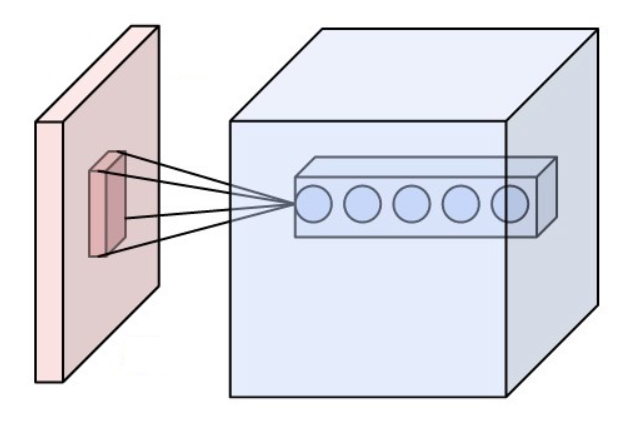
\includegraphics[width=0.4\linewidth]{conv_layer.png}
  \caption{The 2D input image on the right is transformed into a 3D output
  volume by applying multiple convolutions to the input [\cite{conv_layer_wiki}.}]
  \label{fig:conv_layer}
\end{figure}

An interesting example of a CNN outside the realm of image classification is
AtomNet [\cite{dzamba1510atomnet}], which is used to predict bioactivity of
molecules for drug discovery by exploiting the local structure of biochemical
interactions.


\subsection{Gradient Descent}
\label{sub:gradient_descent}

The most common technique to train neural networks is Gradient Descent.
It is based on minimizing a \emph{loss} (cost or penalty) function $\mathcal{L}$
\begin{equation}
  \label{eq:batch_loss}
  \mathcal{L}(\Theta) = \sum_{\vt{u} \in \mathcal{U}} 
                        ||F(\Theta, \vt{u}) - \vt{d}||_2,
\end{equation}
which defines how close the network is to producing the
desired results.  The loss function that is used throughout this thesis is
given by Eq.~\ref{eq:batch_loss}, where the target outputs, given a certain
input $\vec{u}$ out of all training examples $\mathcal{U}$, are denoted by
$\vt{d}$.  

Initially, the weights of the network are set randomly and are to be adjusted
in the optimization phase, also called learning or training.  The loss is, of
course, dependent on all the weights and biases, which is where the gradient
descent comes into play.  The partial derivatives of the loss function are
taken with respect to all the weight and biases of the network to find the
gradient which points in the direction of steepest descent.  With this
calculated direction we can step the weights towards the nearest local minimum
and like that gradually increase the performance of the network.
\begin{equation}
  \label{eq:gradient_descent}
  \Theta' = \Theta + \eta \dd{\mathcal{L}}{\Theta}
\end{equation}
The size of the steps is defined by the \emph{learning rate} $\eta$, which has
to be chosen carefully.  If it is too large, the algorithm will oscillate
around the desired minimum, but if chosen too small, the training times will
become too long.  Several adaptive gradient computation algorithms address this
issue. One promising algorithm is called \emph{Adam} (Adaptive Moment
Estimation) [\cite{ADAM}]. Adam combines adaptive gradient descent methods with
momentum based algorithms [\cite{ADAM}]. Momentum-based optimizers add a fraction
of the previously used weight update to simulate an acceleration of the
gradient descent.  The method of applying the gradient descent algorithm to
multi-layer (deep) neural networks is called \emph{backpropagation} (BP),
because the gradient calculation is started at the last layer and iteratively
propagated back through the whole network by applying the chain rule. A more
detailed description of BP is given in Sec.~\ref{sub:backpropagation}.

There are three different variations of gradient descent, which only differ in
the way the sum in Eq.~\ref{eq:batch_loss} is interpreted.  Summing over all
available training examples $\vt{u}$, namely the whole \emph{batch}, is called
{\em batch GD}. Calculating the loss only for a single randomly chosen example,
is called \emph{stochastic gradient descent} (SGD). The compromise of the two,
mini-batch GD, uses a subset of the training examples, performs a weight
update, and then goes on to the next mini-batch.  Both stochastic and
mini-batch GD end up calculating an approximate loss $L$ from a subset $U
\subset \mathcal{U}$:
\begin{equation}
  \mathcal{L}(\Theta) \approx L(\Theta) = 
    \sum_{\vt{u} \in U} ||F(\Theta, \vt{u}) - \vt{d}||_2,
\end{equation}

which also leads to an approximated gradient. The updates that are performed
with the approximate gradient are hoped to enable the optimizer to jump out of
shallow local minima and saddle points, which is discussed further in the next
paragraph.

\subsubsection{Local Minima of the Error Surface}%
\label{ssub:local_minima_of_the_error_surface}

As BP is a gradient-based method, there is no guarantee at all, that the
algorithm will find the global minimum of the error surface.  To illustrate
this, Fig.~\ref{fig:error_surface_bgd} depicts a two dimensional error surface
with a global and a local minimum.  Depending on where on the surface the
optimization is started, it ends up in the local or global minimum.  It was
shown that for linear activation functions, the error surface contains only a
single minimum, the global one, with all other locations of zero gradient being
saddle points [\cite{BALDI}]. Momentum-based optimizers can find the global
minimum quite efficiently in such cases. However, this cannot be generalized to
the practically used NNs that almost exclusively use non-linear activations.
Optimizers that include momentum like the Adam optimizer can still sometimes
yield better results, as depicted in Fig.~\ref{fig:error_surface_bgd}.  The two
plots both show a two dimensional error surface, where the coordinates $x$ and
$y$ are regarded as the weights that have to be optimized.  The black, dotted
lines show different runs with varying initial values of $x$ and $y$.  The left
plot shows the convergence paths of plain batch GD algorithm as described
above, which converges towards the global minimum in three out of five cases.
As GD is a purely gradient based method, the path always advances in the
direction of steepest descent.  With the more advanced Adam optimizer, the
global minimum is found in four out of five cases. The momentum towards the
global minimum that is gained in the beginning carries the optimization away
from the local minimum.  Of course there are numerous cases where this approach
will not yield a global minimum. Additionally the Adam algorithm is much more
computationally expensive than plain GD and needs more steps, as can be seen
from the denser dots on the black lines.
\begin{figure}
  \begin{minipage}[b]{.49\textwidth}
    \centering
    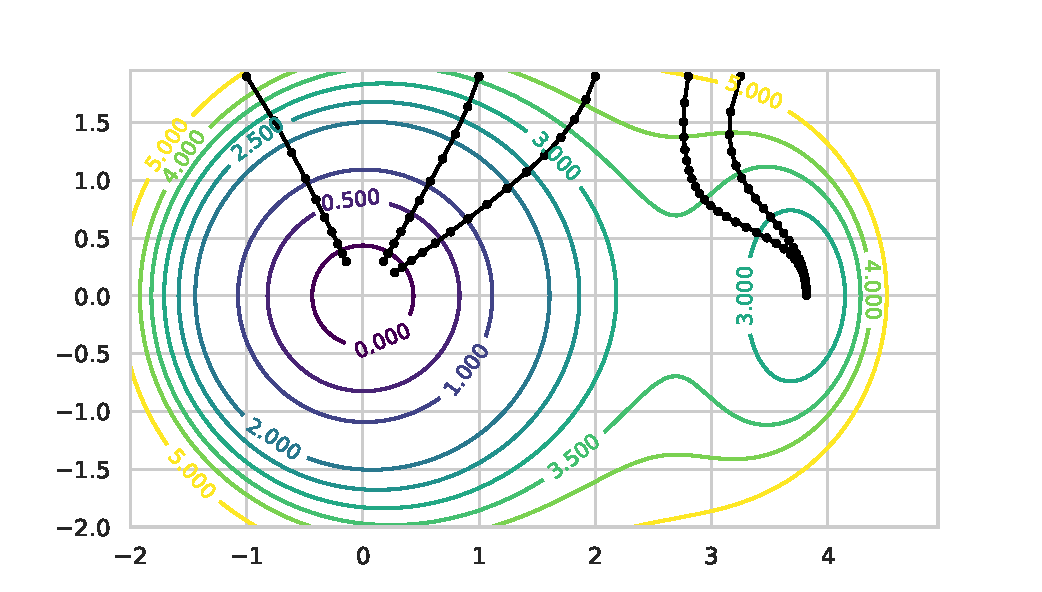
\includegraphics[width=\textwidth]{gradient_descent.pdf}
    GD
  \end{minipage}
  \hspace{.02\textwidth}
  \begin{minipage}[b]{.49\textwidth}
    \centering
    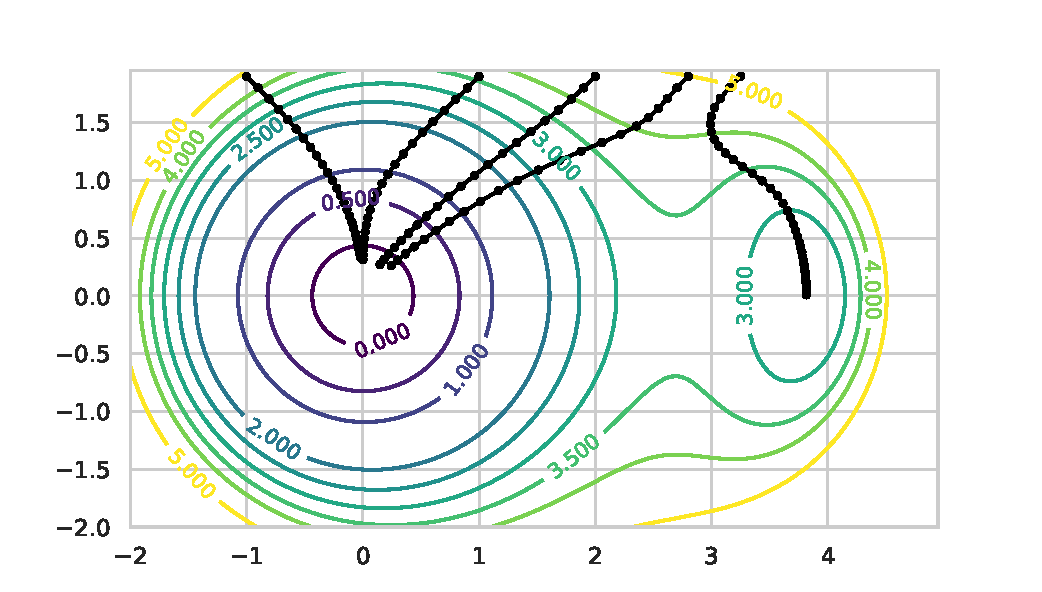
\includegraphics[width=\textwidth]{adam.pdf}
    Adam
  \end{minipage}
  \caption{On the left we can see a plain GD optimizer while on the right the
    Adam optimizer was used.  Depending on the starting values of the two
    variables, there are cases in which the optimization ends in the local
    minimum on the right. The GD optimizer needs fewer steps, while Adam finds
    the global minimum in one more case.}
  \label{fig:error_surface_bgd}
\end{figure}

\begin{figure}
  \begin{minipage}[b]{.49\textwidth}
    \centering
    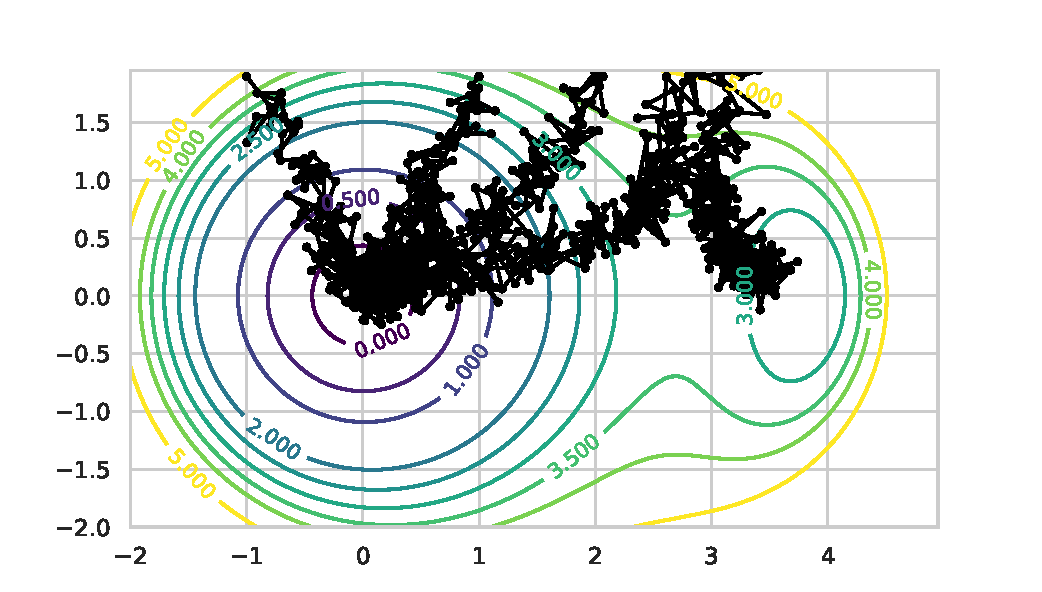
\includegraphics[width=\textwidth]{stochastic_gradient_descent.pdf}
    stochastic GD
  \end{minipage}
  \hspace{.02\textwidth}
  \begin{minipage}[b]{.49\textwidth}
    \centering
    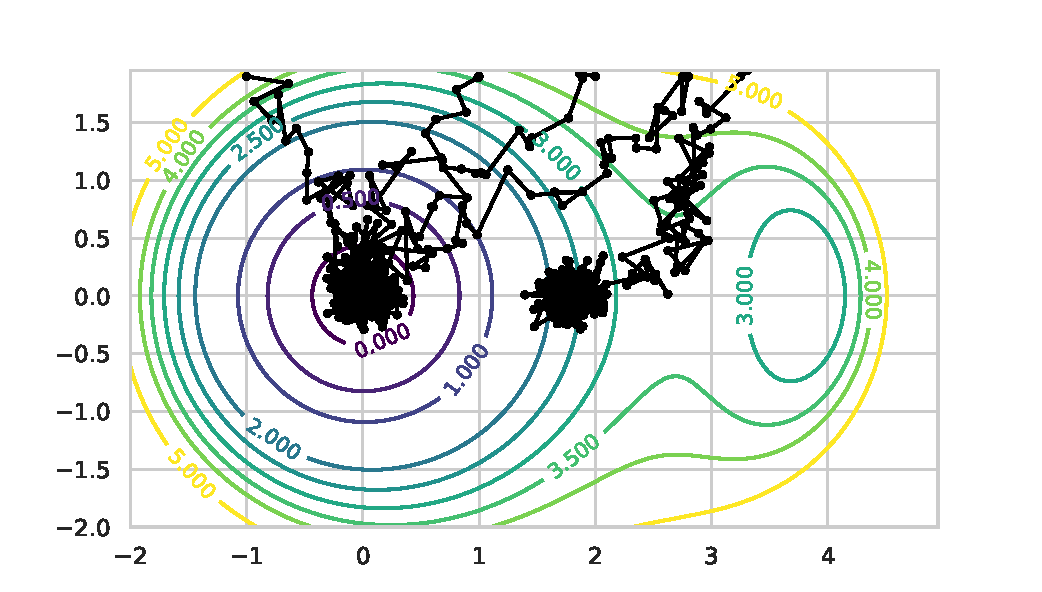
\includegraphics[width=\textwidth]{stochastic_adam.pdf}
    stochastic Adam
  \end{minipage}
  \caption{The plot on the left shows the convergence paths of stochastic plain
    GD, which find the global minimum in on more case compared to batch GD.}
  \label{fig:error_surface_sgd}
\end{figure}
To date, the most commonly used technique to encourage GD to converge to the
global minimum is mini-batch gradient descent.  Instead of evaluating the
\emph{true} loss of the whole training set as indicated by
Eq.~\ref{eq:batch_loss}, SGD adapts the weights after every mini-batch $X$.
This leads to an approximation of the gradient and causes oscillations in the
convergence path, which should make it more probable to escape local minima.
Fig.~\ref{fig:error_surface_sgd} again compares plain GD and Adam, but now with
the perturbing effect of evaluating an approximate loss. The number of training
steps that have to be taken increase significantly, but plain SGD is able to
find the global minimum in four out of five cases now. Stochastic Adam almost
reaches the minimum in all five cases, but seems just get stuck right before
the global minimum in the last case.  The conclusion we can draw from the above
examples is that care has to be taken with respect to the convergence of NNs.
Different optimizers, gradient descent variations, and initializations can
yield vastly different results. However, experience has shown that in most
pattern recognition tasks, SGD algorithms can find a local minimum that yields
satisfactory performance, even though it is not guaranteed that this minimum is
global.  In most applications, an increase in the network connections is
supposed to create paths around suboptimal local minima [\cite{rumelhart1986}].
Additionally, in most application the training is actually stopped early,
meaning at the time the validation error does not decrease further.  This is
done because a network that is fitted perfectly to the training data would most
probably not generalize well over new inputs.  In most cases it is therefore
acceptable or even desirable to remain in a \emph{good} local minimum that
results in a good generalization of the network.


\subsection{Backpropagation}%
\label{sub:backpropagation}

Backpropagation is the basic algorithm that carries out the GD minimizations
that were introduced previously. It was invented in the 1970s but not widely
used until the paper by~[\cite{rumelhart1986}], which marks a breakthrough in the
field of machine learning.  For an easy to read but in depth description of the
subtleties of BP the reader is referred to the book \emph{Neural Networks and
Deep Learning} by [\cite{Nielsen2015}].

Fundamentally, BP is nothing more than the application of the chain rule to the
cost function of a neural network, which can be solved by an \emph{automatic
differentiation} (AD) algorithm. In fact, BP is a special case of AD called
\emph{reverse mode} AD~[\cite{autodiff}].  To illustrate the BP algorithm we will
consider a network with $L$ feedforward layers, where the activations of the
first layer are just the inputs to the network ($\vec{u} = \vec{y}_1$) and the
last layer contains the network outputs $\vec{y}_L$. The components $y^j_l$ of
the vector $\vec{y}_l$ that contains all activations of a layer $l$ are
calculated based on the previous layer:
\begin{equation}
\begin{aligned}
  z^j_l &= \sum_k w^{jk}_l y^k_{l-1} + b^k_L \\
  y^j_l &= \varphi(z^k_l) \label{eq:forward_pass},
\end{aligned}
\end{equation}
where $\vec{z}_l$ are called the \emph{weighted input}.  The system above may
be altered such that a given activation depends on any \emph{previous} layer
activation, but \emph{not} on activations of any \emph{next} layer. This step is
named \emph{forward pass}.  During the forward pass, all activations are
calculated starting from the first layer. The goal of the \emph{backward pass}
is now to adjust all the weights $w^{jk}_l$ (and biases $b^k_L$) such that the loss $L$
\begin{equation}
  L = \frac{1}{2}\sum_k (d^k - y^k_L)^2
\end{equation}
of a single input example $\vec{u}$ is minimized. BP solves this by iteratively
calculating the gradients needed for Eq.~\ref{eq:gradient_descent} starting
from the last layer.  Before directly calculating the necessary gradients it is
easier to compute the \emph{error} $\delta_L$ of the weighted inputs for each
unit $j$ of the last layer:
\begin{equation}
  \delta^j_L = \dd{L}{z^j_L} = \frac{1}{2}\sum_k \dd{}{z^j_L}(d^k - y^k_L)^2
             = \dd{L}{y^j_L}\dd{y^j_L}{z^j_L}
             = (d^j - y^j_L) \varphi'(z^j_L) \label{eq:delta_last_layer},
\end{equation}
where the sum vanishes because $y^k_L$ only depends on $z^j_L$ if $j = k$.
Now the error of any layer $l$ can be expressed in terms of the error of the
next layer $l+1$:
\begin{equation}
  \delta^j_{l} = \dd{L}{z^j_l} = \sum_k \dd{L}{z^j_{l+1}}\dd{z^j_{l+1}}{z^j_l}
  = \sum_k \delta^j_{l+1} \dd{z^j_{l+1}}{z^j_l}
  = \sum_k \delta^j_{l+1} w^{kj}_{l+1} \varphi'(z^j_l) \label{eq:delta_other_layer}
\end{equation}

Now the desired error gradients can be found to be:
\begin{equation}
\begin{aligned}
  \dd{L}{b^j_l} &= \delta^j_l, \\
  \dd{L}{w^{jk}_l} &= y^j_{l-1} \delta^j_l \label{eq:error_grads}
\end{aligned}
\end{equation}
They can now be used to incrementally update the weights and biases according
to Eq.~\ref{eq:gradient_descent}.

\subsubsection{The Backpropagation Algorithm}%
\label{ssub:the_backpropagation_algorithm}

\begin{enumerate}
  \item \emph{Input}: $\vec{u}$ is the activation vector of the first layer
    $\vec{y}_1$
  \item \emph{Forward pass}: Compute activations $\vec{y}_l$ for each
    $l=2,3,...,L$ (Eq.~\ref{eq:forward_pass})
  \item \emph{Output error}: Compute error $\delta_L$ of last layer
    (Eq.~\ref{eq:delta_last_layer})
  \item \emph{Backpropagate}: Compute $\delta_{l-1}$ based on error of layer
    $l$ (Eq.~\ref{eq:delta_other_layer})
  \item \emph{Output}: Obtain the gradients of the cost function
    (Eq.~\ref{eq:error_grads})
\end{enumerate}
